% !TeX root = main.tex

\chapter{Prefix Sum and Histogram}
\glsresetall
\label{chapter:prefixsum}

\section{Prefix Sum}
\label{sec:prefixSum}

Prefix sum is a common kernel used in many applications, e.g., recurrence relations, 
compaction problems, string comparison, polynomial evaluation, histogram, radix sort, and quick sort \cite{blelloch1990prefix}. Prefix sum requires restructuring in order to create an efficient FPGA design.

The prefix sum is the cumulative sum of a sequence of numbers. Given a sequence of inputs $in_n$, the prefix sum $out_n$ is the summation of the first $n$ inputs, namely $out_n = in_0 + in_1 + in_2 + \cdots + in_{n-1} + in_n$. The following shows the computation for the first four elements of the output sequence $out$.
\begin{align*} 
out_0 & = in_0 &\\
out_1 & = in_0 + in_1 &\\
out_2 & = in_0 + in_1 + in_2 \\
out_3 & = in_0 + in_1 + in_2 + in_3 \\
\cdots
\end{align*}

Of course, in practice we don't want to store and recompute the sum of all of the previous inputs, so the prefix sum is often computed by the recurrence equation:
\begin{equation}
out_n = out_{n-1} + in_n
\end{equation}

The disadvantage of the recurrence equation is that we must compute $out_{n-1}$ before computing $out_n$, which fundamentally limits the parallelism and throughput that this computation can be performed.  In contrast, the original equations have obvious parallelism where each output can be computed independently at the expense of a significant amount of redundant computation.  C code implementing the recurrence equation is shown in Figure \ref{fig:prefixsumSW}. Ideally, we'd like to achieve $II=1$ for the loop in the code, but this can be challenging even for such simple code.  Implementing this code with \VHLS results in behavior like that shown in Figure \ref{fig:prefixsumSW}.
\begin{figure}
\begin{minipage}{.5\textwidth}
\lstinputlisting{examples/prefixsumBO.cpp}
\end{minipage}
\begin{minipage}{.5\textwidth}
\centering
\includesvg{prefixsumBO_behavior}
\end{minipage}
\caption{ Code for implementing prefix sum, and its accompanying behavior. }
\label{fig:prefixsumSW}
\end{figure}

The way this code is written, each output is written into the output memory \lstinline|out[]| and then in the next iteration is read back out of the memory again.  Since the memory read is has a latency of one, data read from memory cannot be processed until the following clock cycle.  As a result, such a design can only achieve a loop II of 2.  In this case there is a relatively easy way to rewrite the code: we can simply perform the accumulation on a separate local variable, rather than reading the previous value back from the array.  Avoiding extra memory accesses in favor of register storage is often advantageous in processor code, but in HLS designs it is often more significant since other operations are rarely a performance bottleneck.  Code that does this is shown in Figure \ref{fig:prefixsum_optimized}.

\begin{figure}
\begin{minipage}{.5\textwidth}
\lstinputlisting{examples/prefixsum_optimized.cpp}
\end{minipage}
\begin{minipage}{.5\textwidth}
\centering
\includesvg{prefixsum_optimized_behavior}
\end{minipage}
\caption{ Code for implementing an optimized prefix sum, and its accompanying behavior. }
\label{fig:prefixsum_optimized}
\end{figure}

You might ask why the compiler is not able to optimize the memory loads and stores automatically in order to improve the II of the design.  It turns out that \VHLS is capable of optimizing loads and stores to array, but only for reads and writes within the scope of a single basic block.  You can see this if we unroll the loop, as shown in Figure \ref{fig:prefixsum_unrolled}.  Note that we also have to add appropriate \lstinline{array_partition} s in order to be able to read and write multiple values at the interfaces.   In this case, \VHLS is able to eliminate most of the read operations of the \lstinline{out[]} array within the body of the loop, but we still only achieve a loop II of 2.  In this case the first load in the body of the loop is still not able to be removed.  We can, however, rewrite the code manually to use a local variable rather than read from the \lstinline{out[]} array.

\begin{figure}
\begin{minipage}{.5\textwidth}
\lstinputlisting{examples/prefixsum_unrolled.cpp}
\end{minipage}
\begin{minipage}{.5\textwidth}
\raggedleft
\includesvg{prefixsum_unrolled_behavior}
\end{minipage}
\caption{ Optimizing the prefixsum code using \lstinline{unroll}, \lstinline{pipeline}, and \lstinline{array_partition} directives. }
\label{fig:prefixsum_unrolled}
\end{figure}

%results in the following message:
%\lstinputlisting[basicstyle=\ttfamily\footnotesize]{examples/prefixsumBO.message}

%\begin{figure}
%\lstinputlisting{examples/prefixsumBO.cpp}
%\caption{ The initial code for implementing prefix sum. }
%\label{fig:prefixsumSW}
%\end{figure}

Ideally, when we unroll the inner loop, we the perform more operations per clock and reduce the interval to compute the function. If we unroll by a factor of two, then the performance doubles. A factor of four would increase the performance by factor four, i.e., the performance scales in a linear manner as it is unrolled. While this is mostly the case, as we unroll the inner loop there are often some aspects of the design that don't change.  Under most circumstances, such as when the iteration space of loops execute for a long time, these aspects represent a small fixed overhead which doesn't contribute significantly to the performance of the overall function.  However, as the number of loop iterations decreases, these fixed portions of the design have more impact.  The largest fixed component of a pipelined loop is the depth of the pipeline itself.  The control logic generate by \VHLS for a pipelined loop requires the pipeline to completely flush before code after the loop can execute.

\begin{exercise}
Unroll the \lstinline{for} loop corresponding to the prefix sum code in Figure \ref{fig:prefixsum_optimized} by different factors in combination with array partitioning to achieve a loop II of 1.  How does the \lstinline{prefixsum} function latency change? What are the trends in the resource usages? Why do you think you are seeing these trends? What happens when the loop becomes fully unrolled?
\end{exercise}

\begin{figure}
\centering
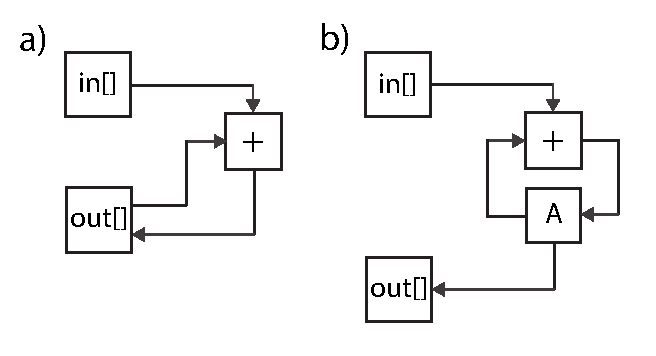
\includegraphics[width=  .7\textwidth]{images/architectures_prefixsum}
\caption{ Part a) displays an architecture corresponding to the code in Figure~\ref{fig:prefixsumSW}. The dependence on the \lstinline{out[]} array can prevent achieving a loop II of 1. Computing the recurrence with a local variable, as shown in the code in Figure~\ref{fig:prefixsum_optimized}, is able to reduce the latency in the recurrence and achieve a loop II of 1.}
\label{fig:architecture_prefixsum}
\end{figure}

Figure~\ref{fig:architecture_prefixsum} shows the hardware architecture resulting from synthesizing the code from Figure \ref{fig:prefixsumSW} and Figure~\ref{fig:prefixsum_optimized}.   In part a), we can see that the `loop' in the circuit includes the output memory that stores the \lstinline{out[]} array, whereas in part b), the loop in the circuit includes only a register that stores the accumulated value and the output memory is only written.  Simplifying recurrences and eliminating unnecessary memory accesses is a common practice in optimizing HLS code.

%This \lstinline{A} variable maps to a hardware register. A register is helpful because a it can be read to and written from on every cycle. Unlike a memory, which has limited number of read and write ports, the register value can be read from and subsequently sent to a large number of places that need that data on every cycle with very limited penalty. The only major issues is wire routing, which in the grand scheme of things is not much additional overhead in terms of resources. Nor does it typically incur a large penalty in terms of performance. 

\note{Could add a whole part about doing reduction. Probably not necessary.}
\note{Should have something here about what to do with floating point accumulation.  This is fundamentally more problematic than what's above (which is relatively easily handled by improving store->load optimization.}

The goal of this section is to show that even a small changes in the code can sometimes have a significant effect on the hardware design. Some changes may not necessarily be intuitive, but can be identified with feedback from the tool.

\section{Histogram}
\label{sec:histogram}

A Histogram models the probability distribution of a discrete signal. Given a sequence of discrete input values, the histogram counts the number of times each value appears in the sequence.  When normalized by the total number of input values, the histogram becomes the probability distribution function of the sequence.  Creating a histogram is a common function used in image processing, signal processing, database processing, and many other domains.  In many cases, it is common to quantize high-precision input data into a smaller number of intervals or \term{bins} as part of the histogram computation.  For the purpose of this section, we will skip the actual process by which this is done and focus on what happens with the binned data.

\begin{figure}
\centering
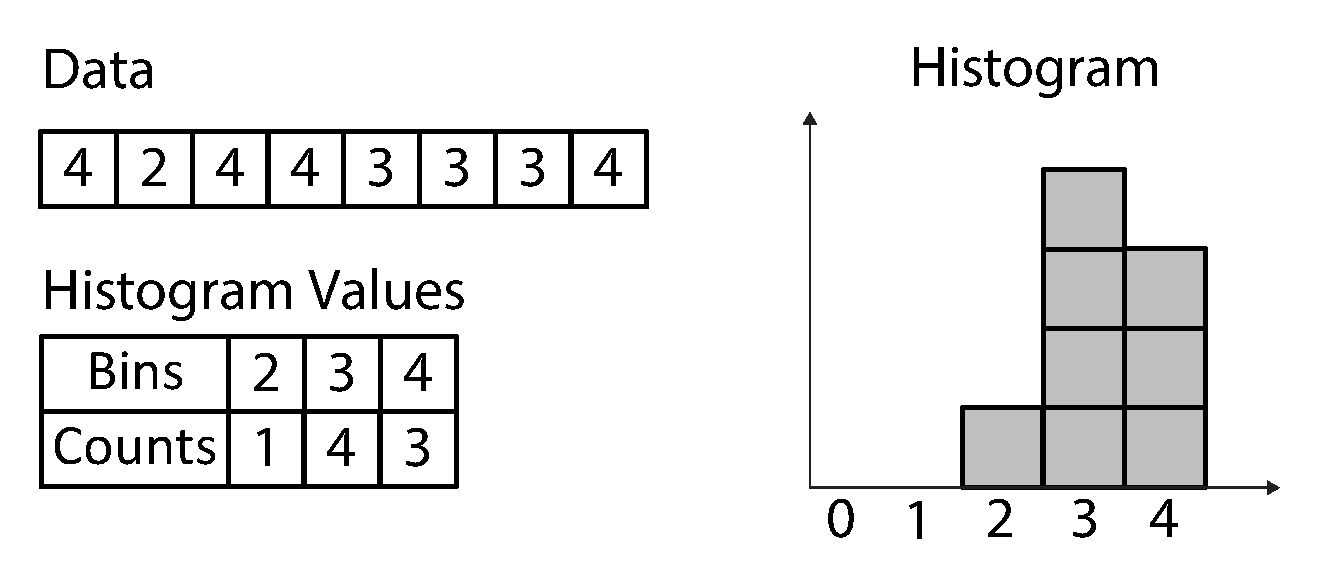
\includegraphics[width=  .7\textwidth]{images/histogram_introd}
\caption{ An example of a histogram.  }
\label{fig:histogram_introd}
\end{figure}

Figure~\ref{fig:histogram_introd} provides a simple example of a histogram.  The data set consists of a sequence of binned values, in this case represented by an integer in $[0,4]$. The corresponding histogram, consisting of a count for each bin, is shown below along with a graphical representation of the histogram, where the height of each bar corresponding to the count of each separate value.  Figure~\ref{fig:histogramSW} shows baseline code for the \lstinline{histogram} function.

\begin{figure}
\lstinputlisting{examples/histogramSW.cpp}
\caption{ Original code for calculating the histogram. The \lstinline{for} loop iterates across the input array and increments the corresponding element of the \lstinline{hist} array. }
\label{fig:histogramSW}
\end{figure}

The code ends up looking very similar to the prefix sum in the previous section.  The difference is that the prefix sum is essentially only performing one accumulation, while in the \lstinline|histogram| function we compute one accumulation for each bin.  The other difference is that in the prefix sum we added the input value each time, in this case we only add 1.  When pipelining the inner loops using the \lstinline|pipeline| directive, we return to the same problem as with the code in Figure \ref{fig:prefixsumSW}, where we can only achieve a loop II of 2 due to the recurrence through the memory.   This is due to the fact that we are reading from the \lstinline{hist} array and writing to the same array in every iteration of the loop.  
Figure~\ref{fig:architecture_histogram} shows the hardware architecture for the code in Figure~\ref{fig:histogramSW}. You can see that the \lstinline{hist} array has a read and write operation. The \lstinline{val} variable is used as the index into the \lstinline{hist} array, and the variable at that index is read out, incremented, and written back into the same location.

\begin{figure}
\centering
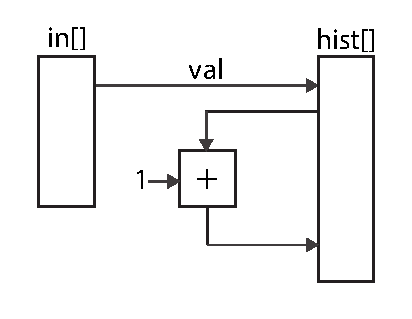
\includegraphics[width=  .5\textwidth]{images/architectures_histogram}
\caption{ An architecture resulting from the code in Figure \ref{fig:histogramSW}. The \lstinline{val} data from the \lstinline{in} array is used to index into the \lstinline{hist} array. This data is incremented and stored back into the same location.}
\label{fig:architecture_histogram}
\end{figure}

\section{Histogram Optimization and False Dependencies}
Let's look deeper at the recurrence here.  In the first iteration of the loop, we read the \lstinline{hist} array at some location $x_0$ and write back to the same location $x_0$.  The read operation has a latency of one clock cycle, so the write has to happen in the following clock.  Then in the next iteration of the loop, we read at another location $x_1$.  Both $x_0$ and $x_1$ are dependent on the input and could take any value, so we consider the worst case when generating the circuit.  In this case, if $x_0 == x_1$, then the read at location $x_1$ cannot begin until the previous write has completed.  As a result, we must alternate between reads and writes.  

It turns out that we must alternate between reads and writes as long as $x_0$ and $x_1$ are independent.  What if they are {\em not} actually independent?  For instance, we might know that the source of data never produces two consecutive pieces of data that actually have the same bin.  What do we do now?  If we could give this extra information to the HLS tool, then it would be able to read at location $x_1$ while writing at location $x_0$ because it could guarantee that they are different addresses.   In \VHLS, this is done using the \lstinline|dependence| directive.

The modified code is shown in Figure \ref{fig:histogram_dependence}.  Here we've explicitly documented (informally) that the function has some preconditions.  In the code, we've added an \lstinline|assert()| call which checks the second precondition.
in \VHLS, this assertion is enabled during simulation to ensure that the simulation testvectors meet the required precondition.  The \lstinline|dependence| directive captures the effect of this precondition on the circuit, generated by the tool.  Namely, it indicates to \VHLS that reads and writes to the \lstinline|hist| array are dependent only in a particular way.  In this case, \lstinline|inter|-iteration dependencies consisting of a read operation after a write operation (RAW) have a distance of 2.  In this case a distance of $n$ would indicate that read operations in iteration $i+n$ only depend on write operations in iteration $i$.  In this case, we assert that \lstinline|in[i+1] != in[i]|, but it could be the case that \lstinline|in[i+2] == in[i]| so the correct distance is 2.

\begin{figure}
\lstinputlisting{examples/histogram_dependence.cpp}
\caption{ An alternative function for computing a histogram.  By restricting the inputs and indicating this restriction to \VHLS via the \lstinline|dependence| directive, II=1 can be achieved without significantly altering the code. }
\label{fig:histogram_dependence}
\end{figure}

\begin{exercise}
In Figure \ref{fig:histogram_dependence}, we added a precondition to the code, checked it using an assertion, and indicated the effect of the precondition to the tool using the \lstinline|dependence| directive.  What happens if your testbench violates this precondition?  What happens if you remove the \lstinline|assert()| call?  Does \VHLS still check the precondition?   What happens if the precondition is not consistent with the \lstinline|dependence| directive?
\end{exercise}

Unfortunately, the \lstinline{dependence} directive doesn't really help us if we are unwilling to accept the additional precondition.  It's also clear that we can't directly apply same optimization as with the \lstinline|prefixsum| function, since we might need to use all of the values stored in the \lstinline|hist| array.  Another alternative is implement the \lstinline|hist| array with a different technology, for instance we could partition the \lstinline|hist| array completely resulting in the array being implemented with \gls{ff} resources.  Since the data written into a \gls{ff} on one clock cycle is available immediately on the next clock cycle, this solves the recurrence problem and can be a good solution when a small number of bins are involved.  The architecture resulting from such a design is shown in Figure \ref{fig:histogram_partitioned}.  However, it tends to be a poor solution when a large number of bins are required.  Commonly histograms are constructed with hundreds to thousands of bins and for large data sets can require many bits of precision to count all of the inputs.   This results in a large number of FF resources and a large mux, which also requires logic resources.  Storing large histograms in \gls{bram} is usually a much better solution.

\begin{figure}
\centering
\note{fixme!}
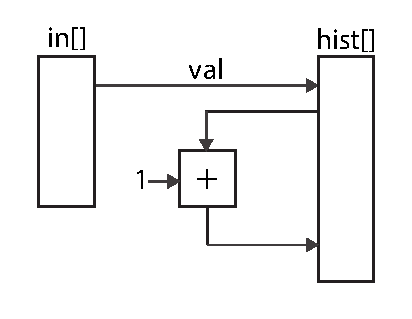
\includegraphics[width=  .5\textwidth]{images/architectures_histogram}
\caption{ An architecture resulting from the code in Figure \ref{fig:histogramSW} when the \lstinline|hist| array is completely partitioned.}
\label{fig:histogram_partitioned}
\end{figure}

Returning to the code in Figure~\ref{fig:histogramSW}, we see that there are really two separate cases that the architecture must be able to handle.  One case is when the input contains consecutive values in the same bin.  In this case, we'd like to use a simple register to perform the accumulation with a minimal amount of delay.  The second case is when the input does not contain consecutive values in the same bin, in which case we need to read, modify, and write back the result to the memory.  In this case, we can guarantee that the read operation of the \lstinline|hist| array can not be affected by the previous write operation.   We've seen that both of these cases can be implemented separately, perhaps we can combine them into a single design.  The code to accomplish this is shown in Figure~\ref{fig:histogramOpt1}. This code uses a local variable \lstinline|old| to store the bin from the previous iteration and another local variable \lstinline{accu} to store the count for that bin.  Each time through the loop we check to see if we are looking at the same bin as the previous iteration.  If so, then we can simply increment \lstinline|accu|.  If not, then we need to store the value in \lstinline|accu| in the \lstinline|hist| array and increment the correct value in the \lstinline|hist| array instead.  In either case, we update \lstinline|old| and \lstinline|accu| to contain the current correct values.  The architecture corresponding to this code is shown in Figure \ref{fig:architecture_histogram_restructured}.  

In this code, we still need a \lstinline|dependence| directive, just as in Figure \ref{fig:histogram_dependence}, however the form is slightly different.  In this case the read and write accesses are to two different addresses in the same loop iteration.  Both of these addresses are dependent on the input data and so could point to any individual element of the \lstinline|hist| array.  Because of this, \VHLS assumes that both of these accesses could access the same location and as a result schedules the read and write operations to the array in alternating cycles, resulting in a loop II of 2.  However, looking at the code we can readily see that \lstinline|hist[old]| and \lstinline|hist[val]| can never access the same location because they are in the \lstinline|else| branch of the conditional \lstinline|if(old == val)|.  Within one iteration (an \lstinline|intra|-dependence) a read operation after a write operation (\lstinline|RAW|) can never occur and hence is a \lstinline|false| dependence.  In this case we are not using the \lstinline|dependence| directive to inform the tool about a precondition of the function, but instead about a property of the code itself. 

\begin{figure}
\lstinputlisting{examples/histogram_opt1.cpp}
\caption{ Removing the read after write dependency from the \lstinline{for} loop. This requires an \lstinline{if/else} structure that may seem like it is adding unnecessary complexity to the design. However, it allows for more effective pipelining despite the fact that the datapath is more complicated. }
\label{fig:histogramOpt1}
\end{figure}

\begin{exercise}
Synthesize the code from Figure \ref{fig:histogramSW} and Figure \ref{fig:histogramOpt1}. What is the initiation interval (II) in each case? What happens when you remove the \lstinline{dependence} directive from the code in Figure \ref{fig:histogramOpt1}? How does the loop interval change in both cases? What about the resource usage?
\end{exercise}

\begin{aside}
For the code in Figure \ref{fig:histogramOpt1}, you might question why a tool like \VHLS cannot determine this property.  In fact, while in some simple cases like this one better code analysis could propagate the \lstinline|if| condition property into each branch, we must accept that there are some pieces of code where properties of memory accesses are actually undecidable.  The highest performance in such cases will only be achieved in a static schedule with the addition of user information.  Several recent research works have looked to improve this by introducing some dynamic control logic into the design\cite{winterstein13dynamic, liu17elasticflow, dai17dynamic}.
\end{aside}

A pictorial description of the restructured code from Figure \ref{fig:histogramOpt1} is shown in Figure \ref{fig:architecture_histogram_restructured}. Not all of the operations are shown here, but the major idea of the function is there. You can see the two separate \lstinline{if} and \lstinline{else} regions (denoted by dotted lines). The \lstinline{acc} variable is replicated twice in order to make the drawing more readable; the actual design will only have one register for that variable.  The figure shows the two separate datapaths for the \lstinline{if} and the \lstinline{else} clause with the computation corresponding to the \lstinline{if} clause on the top and the \lstinline{else} clause datapath on the bottom. 

\begin{figure}
\centering
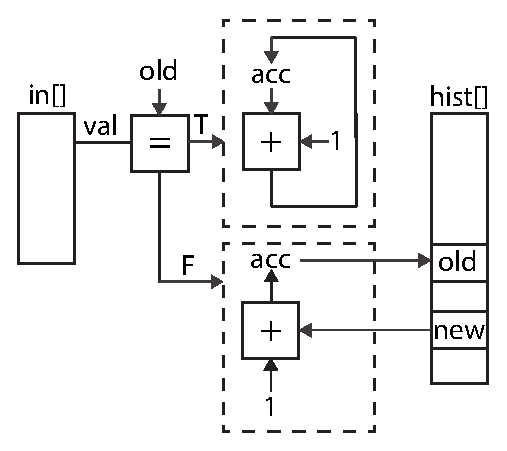
\includegraphics[width=  .6\textwidth]{images/architectures_histogram_restructured}
\caption{ A depiction of the datapath corresponding to the code in Figure \ref{fig:histogramOpt1}. There are two separate portions corresponding to the \lstinline{if} and \lstinline{else} clauses. The figure shows the important portions of the computation, and leaves out some minor details. }
\label{fig:architecture_histogram_restructured}
\end{figure}

\section{Increasing Histogram Performance}

With some effort, we've achieved a design with a loop II of 1.  Previously we have seen how further reducing the execution time of a design can be achieved by partial unrolling of the inner loop.  However, with the \lstinline|histogram| function this is somewhat difficult for several reasons.  One reason is the challenging recurrence, unless we can break up the input data in some fashion, the computation of one iteration of the loop must be completed with the computation of the next iteration of the loop. A second reason is that with a loop II of 1, the circuit performs a read and a write of the \lstinline|hist| array each clock cycle, occupying both ports of a \gls{bram} resource in the FPGA.   Previously we have considered \gls{arraypartitioning} to increase the number of memory ports for accessing an array, but there's not a particularly obvious way to partition the \lstinline|hist| array since the access order depends on the input data.

All is not lost, however, as there is a way we can expose more parallelism by decomposing the histogram computation into two stages.  In the first stage, we divide the input data into a number of separate partitions.  The histogram for each partition can be computed independently using a separate instance, often called a \gls{pe}, of the histogram solution we've developed previously.  In the second stage, the individual histograms are combined to generate the histogram of the complete data sets.  This partitioning (or mapping) and merging (or reducing) process is very similar to that adopted by the MapReduce framework \cite{dean08mapreduce} and is a common pattern for parallel computation.  The map-reduce pattern is applicable whenever there is recurrence which includes a commutative and associative operation, such as addition in this case. This idea is shown in Figure~\ref{fig:architecture_histogram_parallel}. 

\begin{figure}
\centering
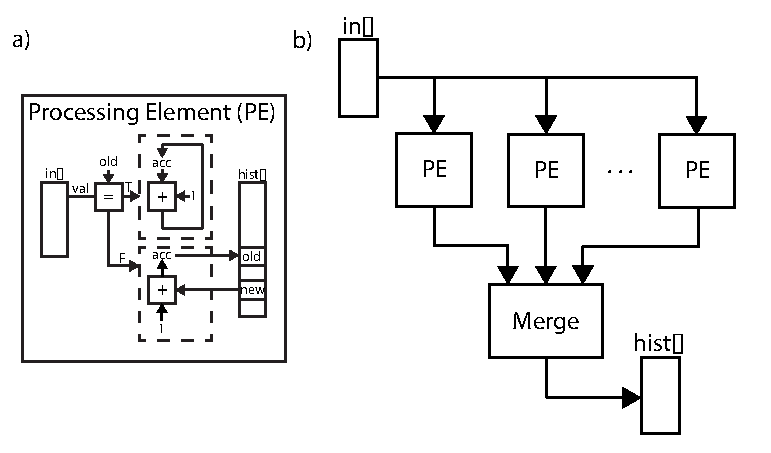
\includegraphics[width=  .9\textwidth]{images/architectures_histogram_parallel}
\caption{The histogram computation implemented using a map-reduce pattern.  The processing element (PE) in Part a) is the same architecture as shown in Figure \ref{fig:architecture_histogram_restructured}. The \lstinline|in| array is partitioned and each partition is processed by a separate \gls{pe}. The merge block combines the individual histograms to create the final histogram.  }
\label{fig:architecture_histogram_parallel}
\end{figure}

The code for implementing this architecture is shown in Figure \ref{fig:histogram_parallel}. The \lstinline{histogram_map} function implements the `map' portion of the map-reduce pattern and will be instantiated multiple times. The code is very similar to the code in Figure \ref{fig:histogramOpt1}. The main difference is that we have added the additional code to initialize the \lstinline|hist| array.  The \lstinline{histogram_map} function takes an input array \lstinline{in} which will contain a partition of the data being processed and computes the histogram of that partition in the \lstinline|hist| array.   The \lstinline{histogram_reduce} function implements the `reduce' portion of the pattern.  It takes as input a number of partial histograms and combines them into complete histogram by adding together the count for each histogram bin.  In our code example in Figure \ref{fig:histogram_parallel}, we have only two processing elements, thus the merge has two input arrays \lstinline{hist1} and \lstinline{hist2}. This can easily be extended to handle more processing elements.

The new \lstinline{histogram} function takes as an input two partitions of the input data, stored in the \lstinline{inputA} and \lstinline{inputB} arrays.  It computes the histogram of each partition using the \lstinline {histogram_map} function, which are then stored in the \lstinline{hist1} and \lstinline{hist2} arrays. These are feed into the \lstinline{histogram_reduce} function which combines them and stores the result in the \lstinline{hist} array, which is the final output of the top level function \lstinline{histogram}. 

\begin{figure}
\lstinputlisting{examples/histogram_parallel.cpp}
\caption{ Another implementation of histogram that uses task level parallelism and pipelining. The histogram operation is split into two sub tasks, which are executed in the two \lstinline{histogram_map} functions. These results are combined in the final histogram result using the \lstinline{histogram_reduce} function. The \lstinline{histogram} function is the top level function that connects these three functions together. }
\label{fig:histogram_parallel}
\end{figure}

\begin{exercise}
Modify the code in Figure \ref{fig:histogram_parallel} to support a parameterizable number \lstinline|NUM_PE| of \glspl{pe}? Hint: You'll need to combine some of the arrays into a single array that is correctly partitioned and add some loops that depend on \lstinline|NUM_PE|.  What happens to the throughput and task interval as you vary the number of \glspl{pe}? 
\end{exercise}

We use the \lstinline{dataflow} directive in the \lstinline{histogram} function in order to enable a design with \gls{taskpipelining}.   In this case there are three processes: two instances of the \lstinline{histogram_map} function and one instance of the \lstinline{histogram_reduce} function. Within a single task, the two \lstinline{histogram_map} processes can execute concurrently since they work on independent data, while the \lstinline{histogram_reduce} function must execute after since it uses the results from the  \lstinline{histogram_map} processes. Thus, the \lstinline{dataflow} directive essentially creates a two stage task pipeline with the \lstinline{histogram_map} functions in the first stage and the \lstinline{histogram_reduce} function in the second stage.   As with any dataflow design, the interval of the entire \lstinline{histogram} function depends upon the maximum initiation interval of the two stages. The two \lstinline{histogram_map} functions in the first stage are the same and will have the same interval ($II_\mathrm{histogram\_map}$). The \lstinline{histogram_reduce} function will have another interval ($II_\mathrm{histogram\_reduce}$). The interval of the toplevel \lstinline{histogram} function $II_\mathrm{histogram}$ is then $\max (II_\mathrm{histogram\_map}, II_\mathrm{histogram\_reduce})$.

\begin{exercise}
What happens when you add or change the locations of the \lstinline{pipeline} directives? For example, is it beneficial to add a \lstinline{pipeline} directive to the \lstinline{for} loop in the \lstinline{histogram_reduce} function? What is the result of moving the \lstinline{pipeline} directive into the \lstinline{histogram_map} function, i.e., hoisting it outside of the \lstinline{for} loop where it currently resides? 
\end{exercise}

The goal of this section was to walk through the optimization the histogram computation, another small but important kernel of many applications. The key takeaway is that there are often limits to what tools can understand about our programs.  In some cases we must take care in how we write the code and in other cases we must actually give the tool more information about the code or the environment that the code is executing in.  In particular, properties about memory access patterns often critically affect the ability of HLS to generate correct and efficient hardware.  In \VHLS, these properties can be expressed using the \lstinline|dependence| directive.  Sometimes these optimizations might even be counter-intuitive, such as the addition of the \lstinline{if/else} control structure in \ref{fig:histogramOpt1}.  In other cases optimizations might require some creativity, as in applying the map-reduce pattern in Figures \ref{fig:architecture_histogram_parallel} and \ref{fig:histogram_parallel}.  

\section{Conclusion}
In this section, we've looked at the prefix sum and histogram kernels.  Although these functions seem different, they both contain recurrences through a memory access.  These recurrences can limit throughput if the memory access is not pipelined.  In both cases, by rewriting the code we can remove the recurrence.  In the case of the prefix sum, this is much easier since the access patterns are deterministic.  In the case of the histogram we must rewrite the code to address the recurrence or ensure that recurrence never happens in practice.   In either case we needed a way to describe to \VHLS information about the environment or about the code itself that the tool was unable to determine for itself.  This information is captured in the \lstinline{dependence} directive.  Lastly, we looked at ways of parallelizing both algorithms yet further, so that they could process a number of data samples each clock cycle.